\documentclass[12pt]{article}
\usepackage[utf8]{inputenc}	
\usepackage[catalan]{babel}
\usepackage{subcaption}
\usepackage[obeyspaces]{url}
\usepackage[colorinlistoftodos]{todonotes}
\usepackage[]{mcode}
\usepackage{fancyvrb}
\usepackage{eurosym} %Símbol del euro
\usepackage[obeyspaces]{url} %PATH
\usepackage{wrapfig} %Imatges WRAP (mateixa linia)
\usepackage[toc,page]{appendix}
\usepackage{todonotes}
\usepackage{appendix}
\usepackage{scrextend}
\usepackage{enumitem}
\usepackage{dirtytalk}
\usepackage{multicol}
\usepackage{listingsutf8}
\usepackage{dirtytalk}

\setlength{\parindent}{0cm} \setlength{\oddsidemargin}{-0.5cm} \setlength{\evensidemargin}{-0.5cm}
\setlength{\textwidth}{17cm} \setlength{\textheight}{23cm} \setlength{\topmargin}{-1cm} \addtolength{\parskip}{2ex}

\definecolor{backcolour}{rgb}{0.95,0.95,0.92}
\lstdefinelanguage{json}{
	backgroundcolor=\color{backcolour},   
	breaklines=true, 
    string=[s]{"}{"},
    stringstyle=\color{blue},
    comment=[l]{:},
    commentstyle=\color{black}
}

\renewcommand{\baselinestretch}{1.5}

\begin{document}
\begin{titlepage}
		\centering
		\includegraphics[width=0.5\textwidth]{imatges/logo3.png}\par\vspace{1cm}
		{\huge\bfseries Posicionament de restaurants\par}
		\vspace{0.3cm}
		{\scshape\Large Processament de Dades Espaials\par}
		\vspace{0.2cm}
		{\scshape\Large Màster en enginyeria informàtica\par}
		\vspace{1.5cm}
		{\Large\itshape Oscar Galera Alfaro i Meriem Abjil Bajja\par}
		\vfill
		{\large \today\par}
\end{titlepage}
\tableofcontents

\clearpage

\listoffigures

\clearpage

\section{Introducció}

Els imaginadors de Disney han descobert com mantenir el seu univers feliç el més petit possible: mitjançant l'ús de polseres \textit{Magic Bands} per fer un seguiment de les identitats, els moviments i l'estat financer dels usuaris.

El MyMagic + "sistema de gestió de vacances" pot fer un seguiment dels convidats a mesura que es mouen per Disney Land Paris i analitzar els seus hàbits de compra.

Degut a l'èxit generat de Disney Land Paris, el propietari de Disney Land Paris ha decidit obrir un nou parc temàtic similar a Disney Land París (\ref{fig:disney1}) en el territori Gironí. Ens han encarregat indicar el posicionament dels restaurants amb l'objectiu de maximitzar els beneficis generats per aquests. Per ubicar aquests restaurants, es realitzarà un estudi de la popularitat de les atraccions que hi ha a DLP a fi de determinar les zones més visitades i d'aquesta manera, fer la distribució dels restaurants més cars en aquestes zones per maximitzar els beneficis del parc.

%Posicionament de la imatge
\begin{figure}[h!]
    \centering
    \includegraphics[width=0.90\textwidth]{imatges/mapa_disney_land_paris.jpg}\par\vspace{1cm}
    \caption{Mapa de Disney Land Paris}
    \label{fig:disney1}
\end{figure}

\clearpage
\section{Objectiu}
L'objectiu del projecte és \textbf{fer la distribució dels restaurants més cars donades unes determinades zones per maximitzar els beneficis del parc}. Aquestes zones són zones candidates, on es poden posar restaurants, del mapa d'atraccions del territori gironí.

Per dur a terme aquest objectiu considerem que el mapa d'atraccions del nou territori és el mateix que el de DLP; que les \textit{Magic Bands} (\ref{fig:magic_bands}) recullen i emmagatzemen la informació de la posició dels seus usuaris cada 5 minuts, i que disposem de tantes zones candidates o més com restaurants volguem ubicar. 

Per determinar el grau d'interès de cada atracció, comptem amb una gran quantitat de dades generades per les \textit{Magic Bands} (\ref{fig:magic_bands}) que es reparteixen a l'entrada del parc temàtic, i que tenen per objectiu l'estudi del comportament del públic. 

\begin{figure}[h]
    \centering
    \includegraphics[width=0.75\textwidth]{imatges/magic_bands.jpg}\par\vspace{1cm}
    \caption{Magic Bands}
    \label{fig:magic_bands}
\end{figure}

\clearpage
%\section{Formalització}
%Bla bla bla
%\subsection{Glossari}
%Bla bla bla
\section{Definició del problema}
Per realitzar l'objectiu del nostre projecte, es distribuirà el procés de realitzar distribució dels restaurants més cars donades unes determinades zones per maximitzar els beneficis del parc en 5 passos:
\begin{enumerate}
	\item Donarem un pes a cada atracció
	\item Repartir el mapa en àrees
	\item Càlcul de la importància de cada atracció
	\item Definir les zones candidates
	\item Ubicar els restaurants
\end{enumerate}

\subsection{Donarem un pes a cada atracció}
El pes d'una atracció el definirem a parir de la quantitat de gent que ha pujat a una atracció. A la figura \ref{fig:mapa_areas}, podem veure el mapa de les atracions amb els pesos de cada atracció.

\begin{figure}[h!]
	\centering
	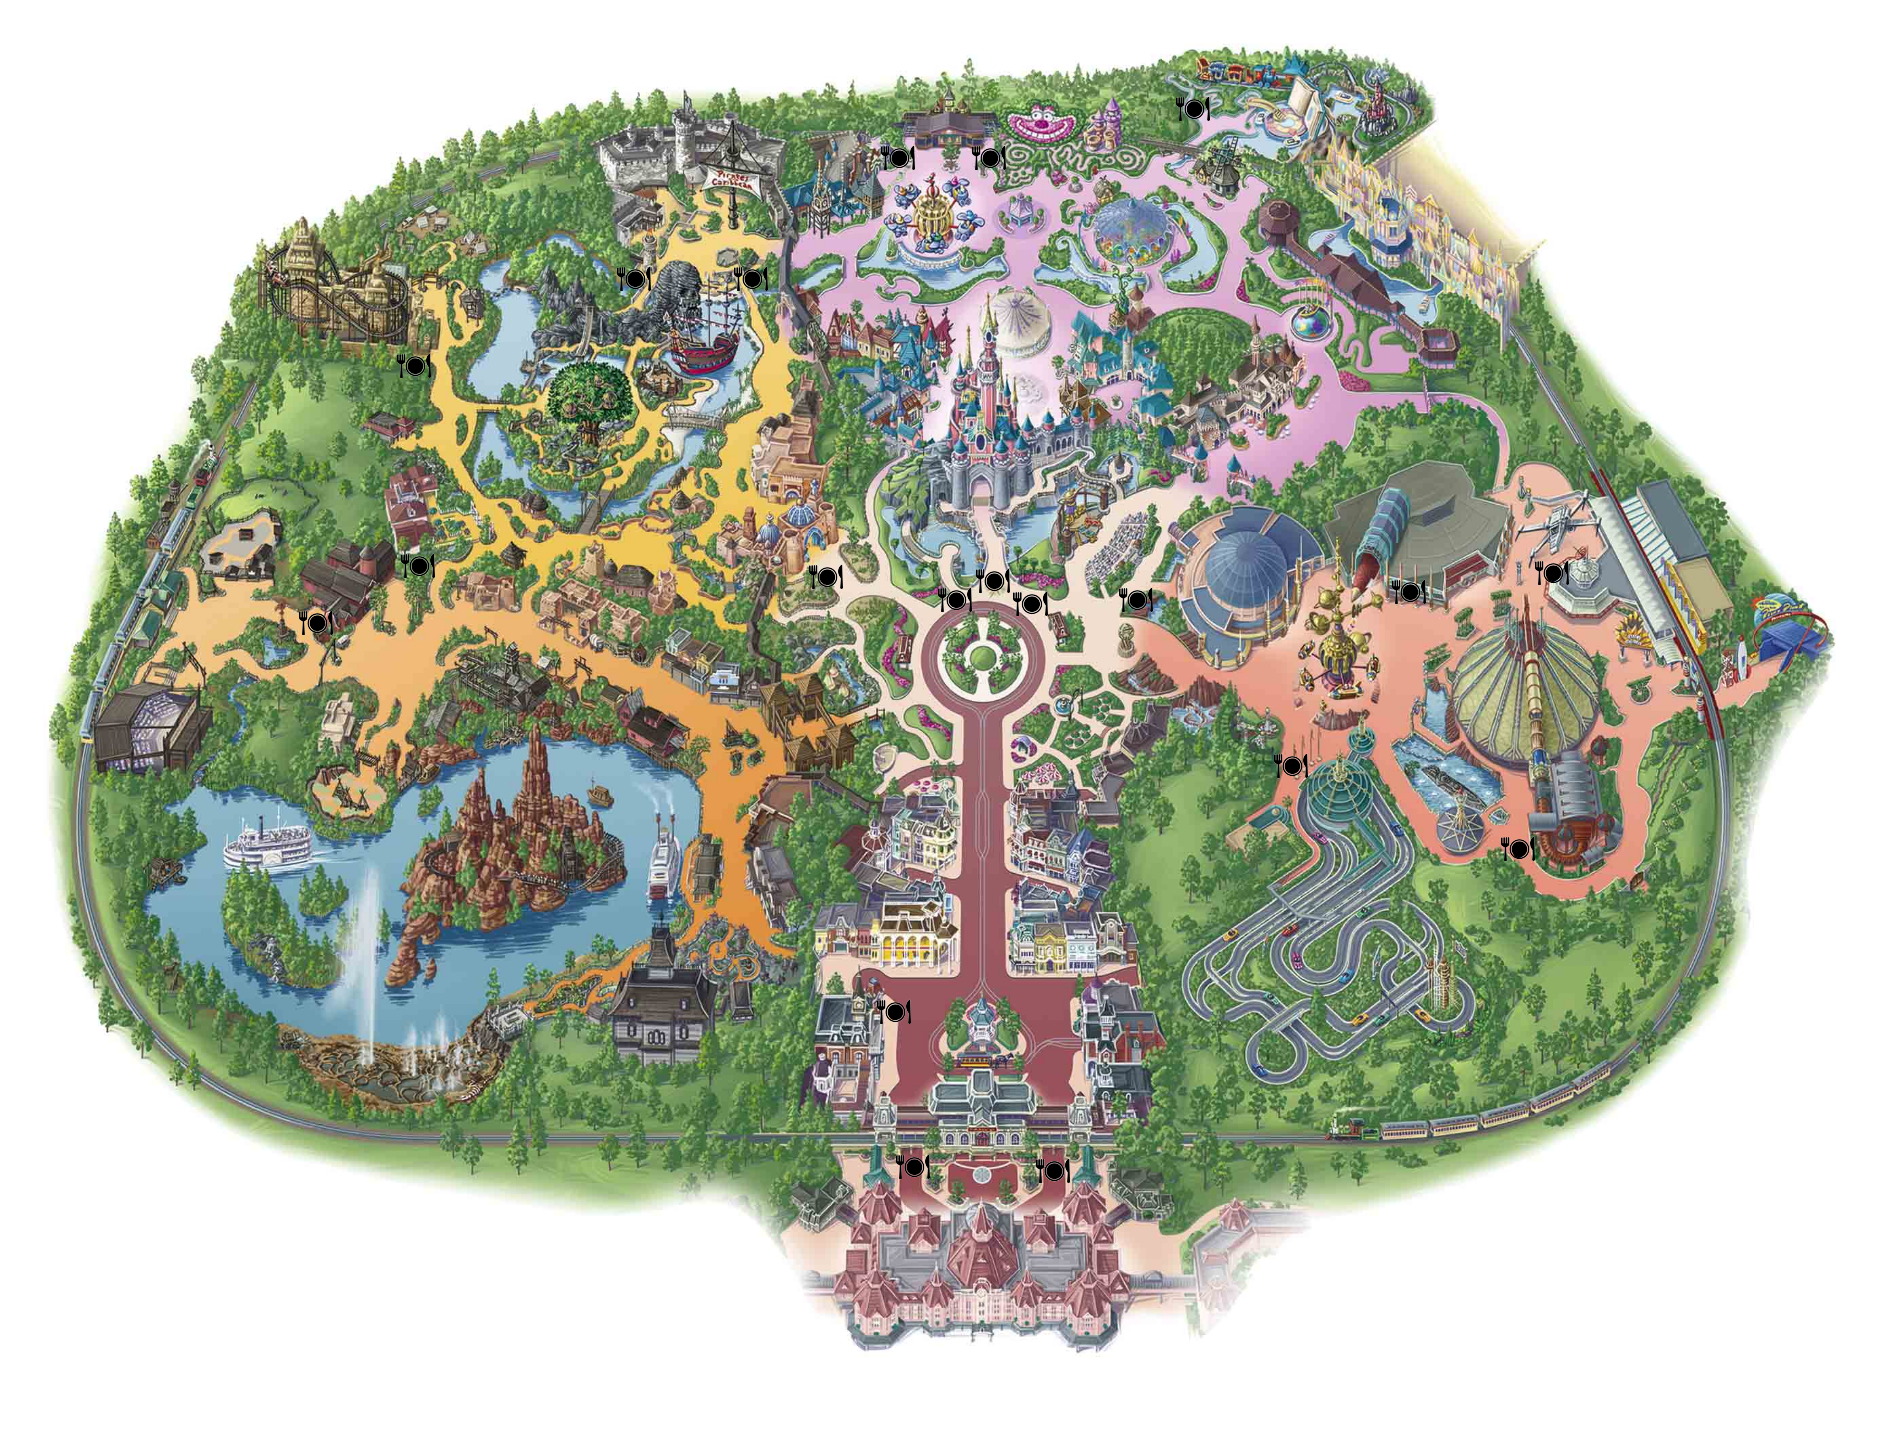
\includegraphics[width=0.5\textwidth]{imatges/mapa_restaurants.png}\par\vspace{1cm}
	\caption{Pesos de cada atracció}
	\label{fig:mapa_areas}
\end{figure}

\subsection{Repartir el mapa en àrees}
Una vegada tenim els pesos de totes les atraccions, realitzarem un diagrama de Voronoi (figura \ref{fig:diagrama_voronoi_ordre_1}), tenint en compte que els pivots estan situats sobre les entrades de les atraccions i el pes del pivot és el pes de l’atracció (nombre de visitants en un període de temps).
		
Això és fa perquè volem tenir el mapa repartit en àrees, on cada àrea representa la regió d’influència de l’atracció. 

\begin{figure}[h!]
	\centering
	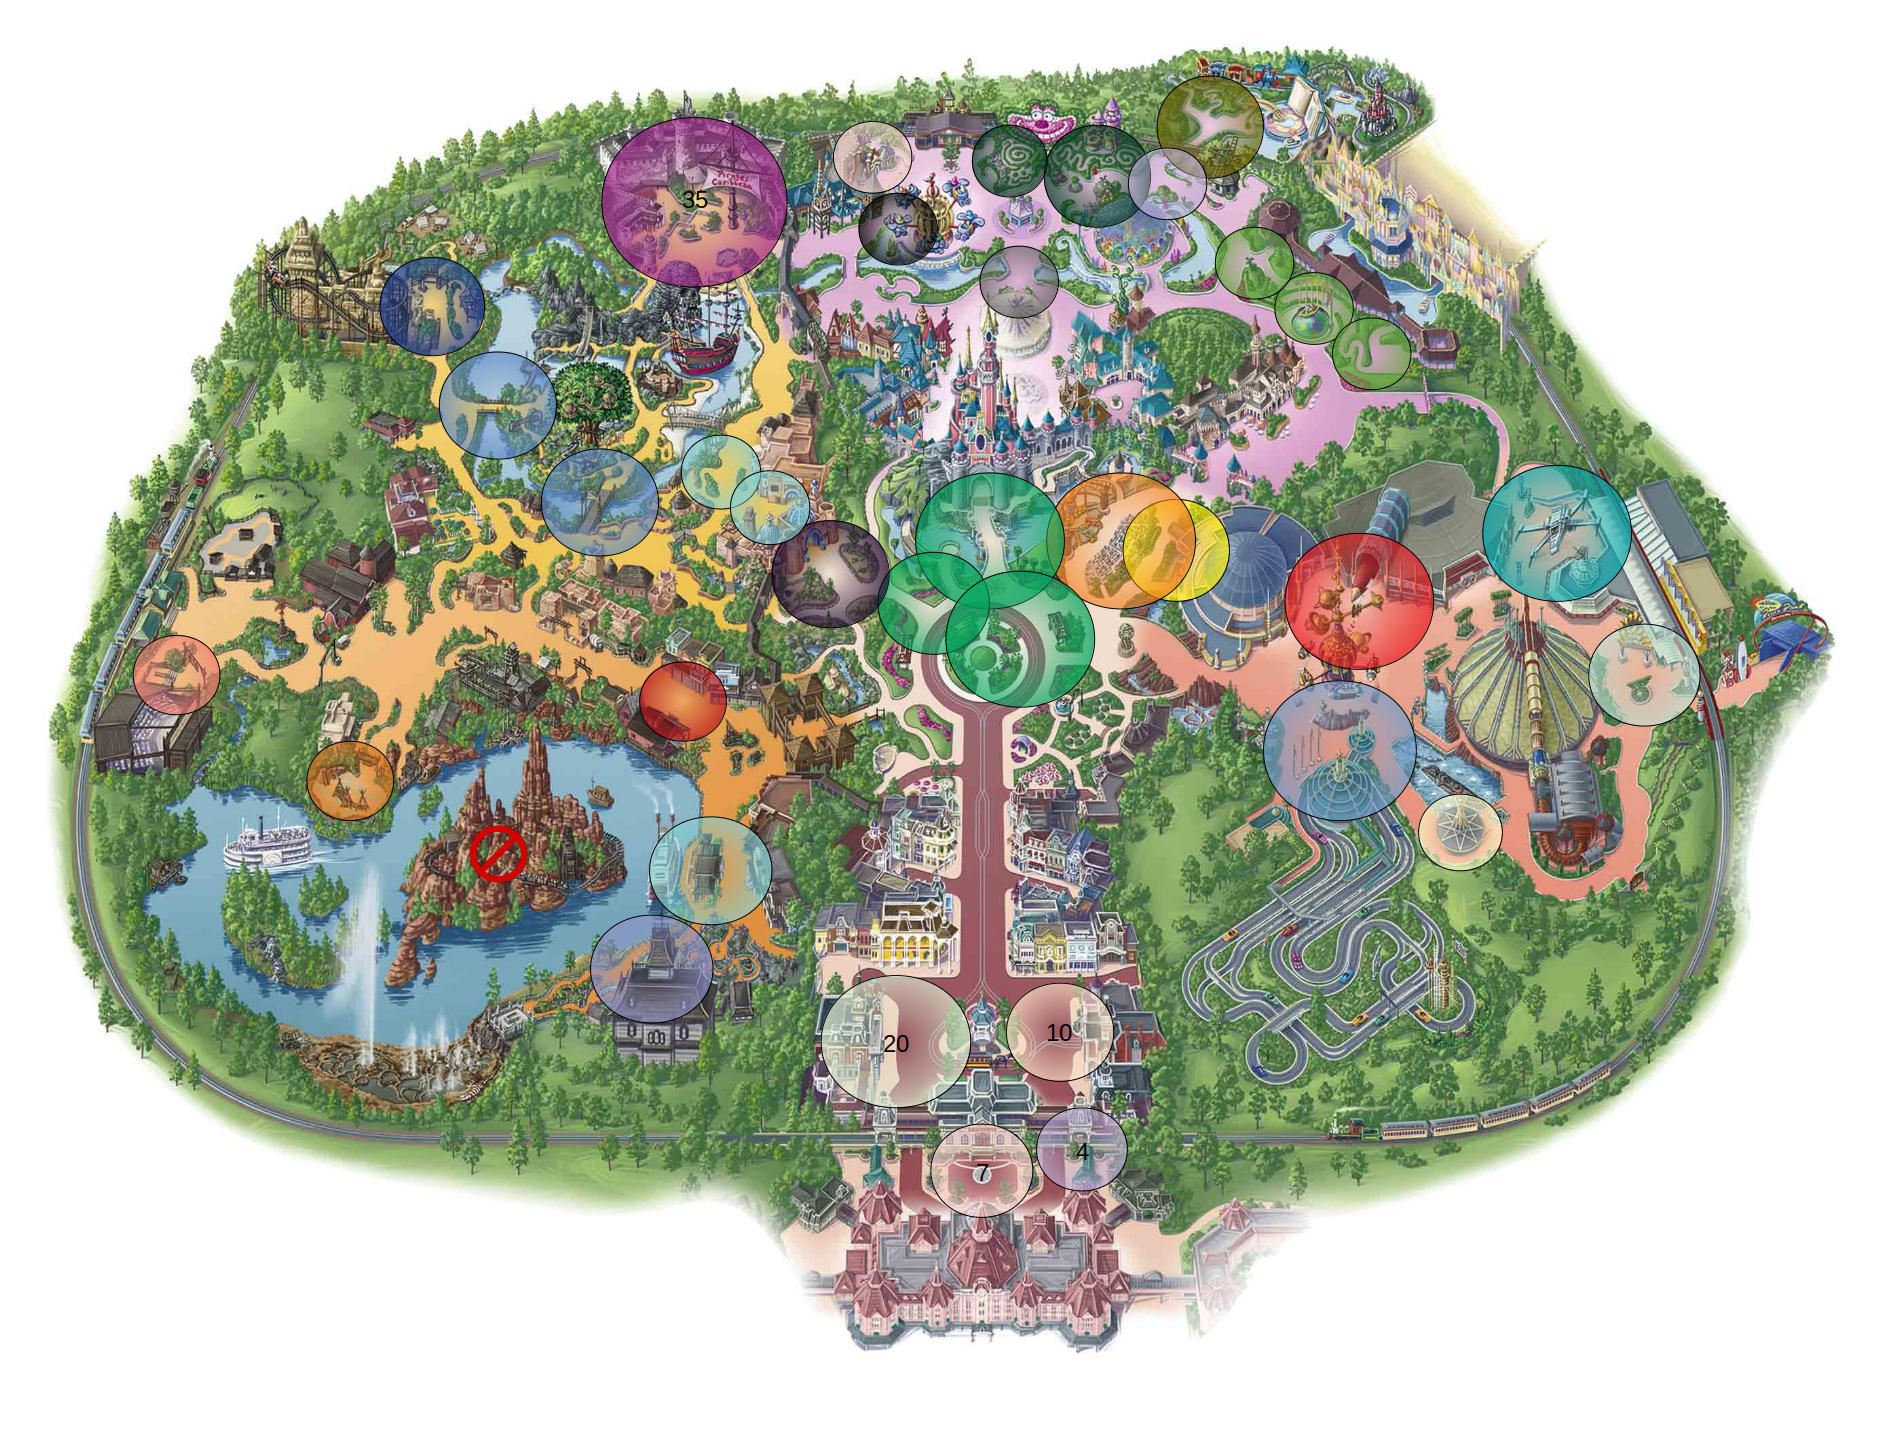
\includegraphics[width=0.5\textwidth]{imatges/diagrama_voronoi_ordre_1.png}\par\vspace{1cm}
	\caption{Diagrama de Voronoi d'ordre 1 considerant que els pivots estan situades sobre les atraccions i el pes del pivot és el pes de l'atracció, nombre de visitants en un període de temps}.
	\label{fig:diagrama_voronoi_ordre_1}
\end{figure}

\subsection{Càlcul de la importància de cada atracció}
Una vegada tenim les àrees de les atraccions definides, calcularem la importància de l’atracció.

Per calcular la importància de l'atracció (i), realitzarem un diagrama de Voronoid d'ordre $k$ ($2 \le k \le 3$) (figura \ref{fig:diagrama_voronoi_ordre_2}) tenint en compte que els pivots estan situats sobre les entrades de les atraccions i el pes del pivot és el pes de l’atracció. 

Llavors la importància d'una atraccio (i) la definim com el sumatori dels punts que es troben a l'àrea definida per l’atracció (trobada amb el diagrama de Voronoi d'ordre 1) + els punts que estan situats només a la capa 2 i els dividirem per la distància al pivot de l'atracció.

\begin{figure}[h!]
	\centering
	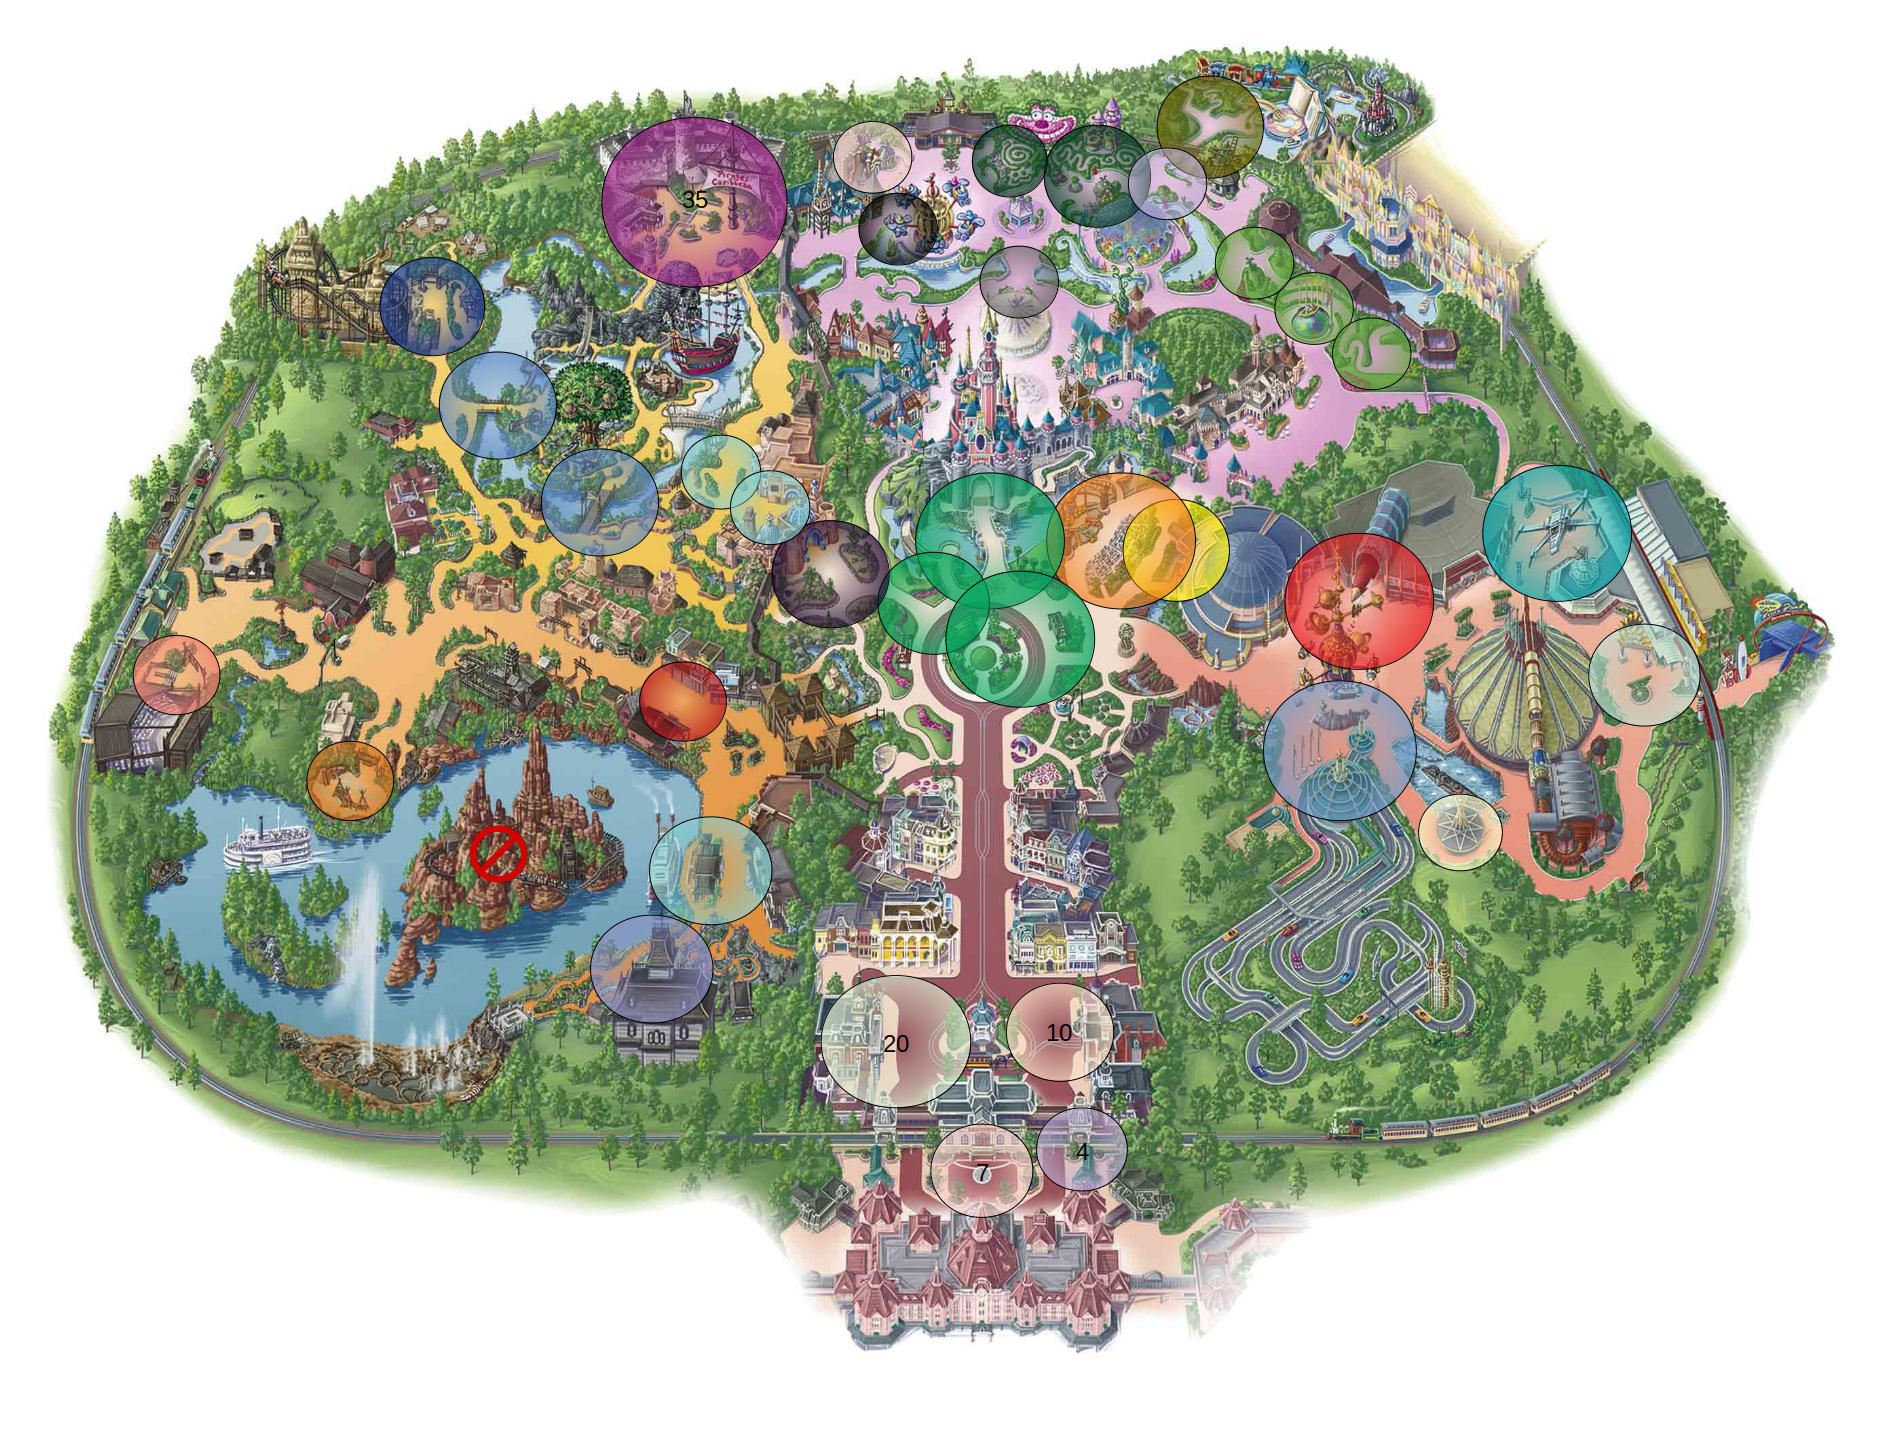
\includegraphics[width=0.5\textwidth]{imatges/diagrama_voronoi_ordre_2.png}\par\vspace{1cm}
	\caption{Diagrama de Voronoi d'ordre $k$ ($2 \le k \le 3$) considerant que els pivots estan situades sobre les atraccions i el pes del pivot és el pes de l'atracció, nombre de visitants en un període de temps}.
	\label{fig:diagrama_voronoi_ordre_2}
\end{figure}

\subsection{Definir les zones candidates}
A partir del diagrama de voronoi anterior, que corresponont a la figura \ref{fig:diagrama_voronoi_ordre_1}, definim els punts on poden anar els restaurants (zones candidates) com es pot observar a la figura \ref{fig:zones_candidates}.

\begin{figure}[h]
	\centering
	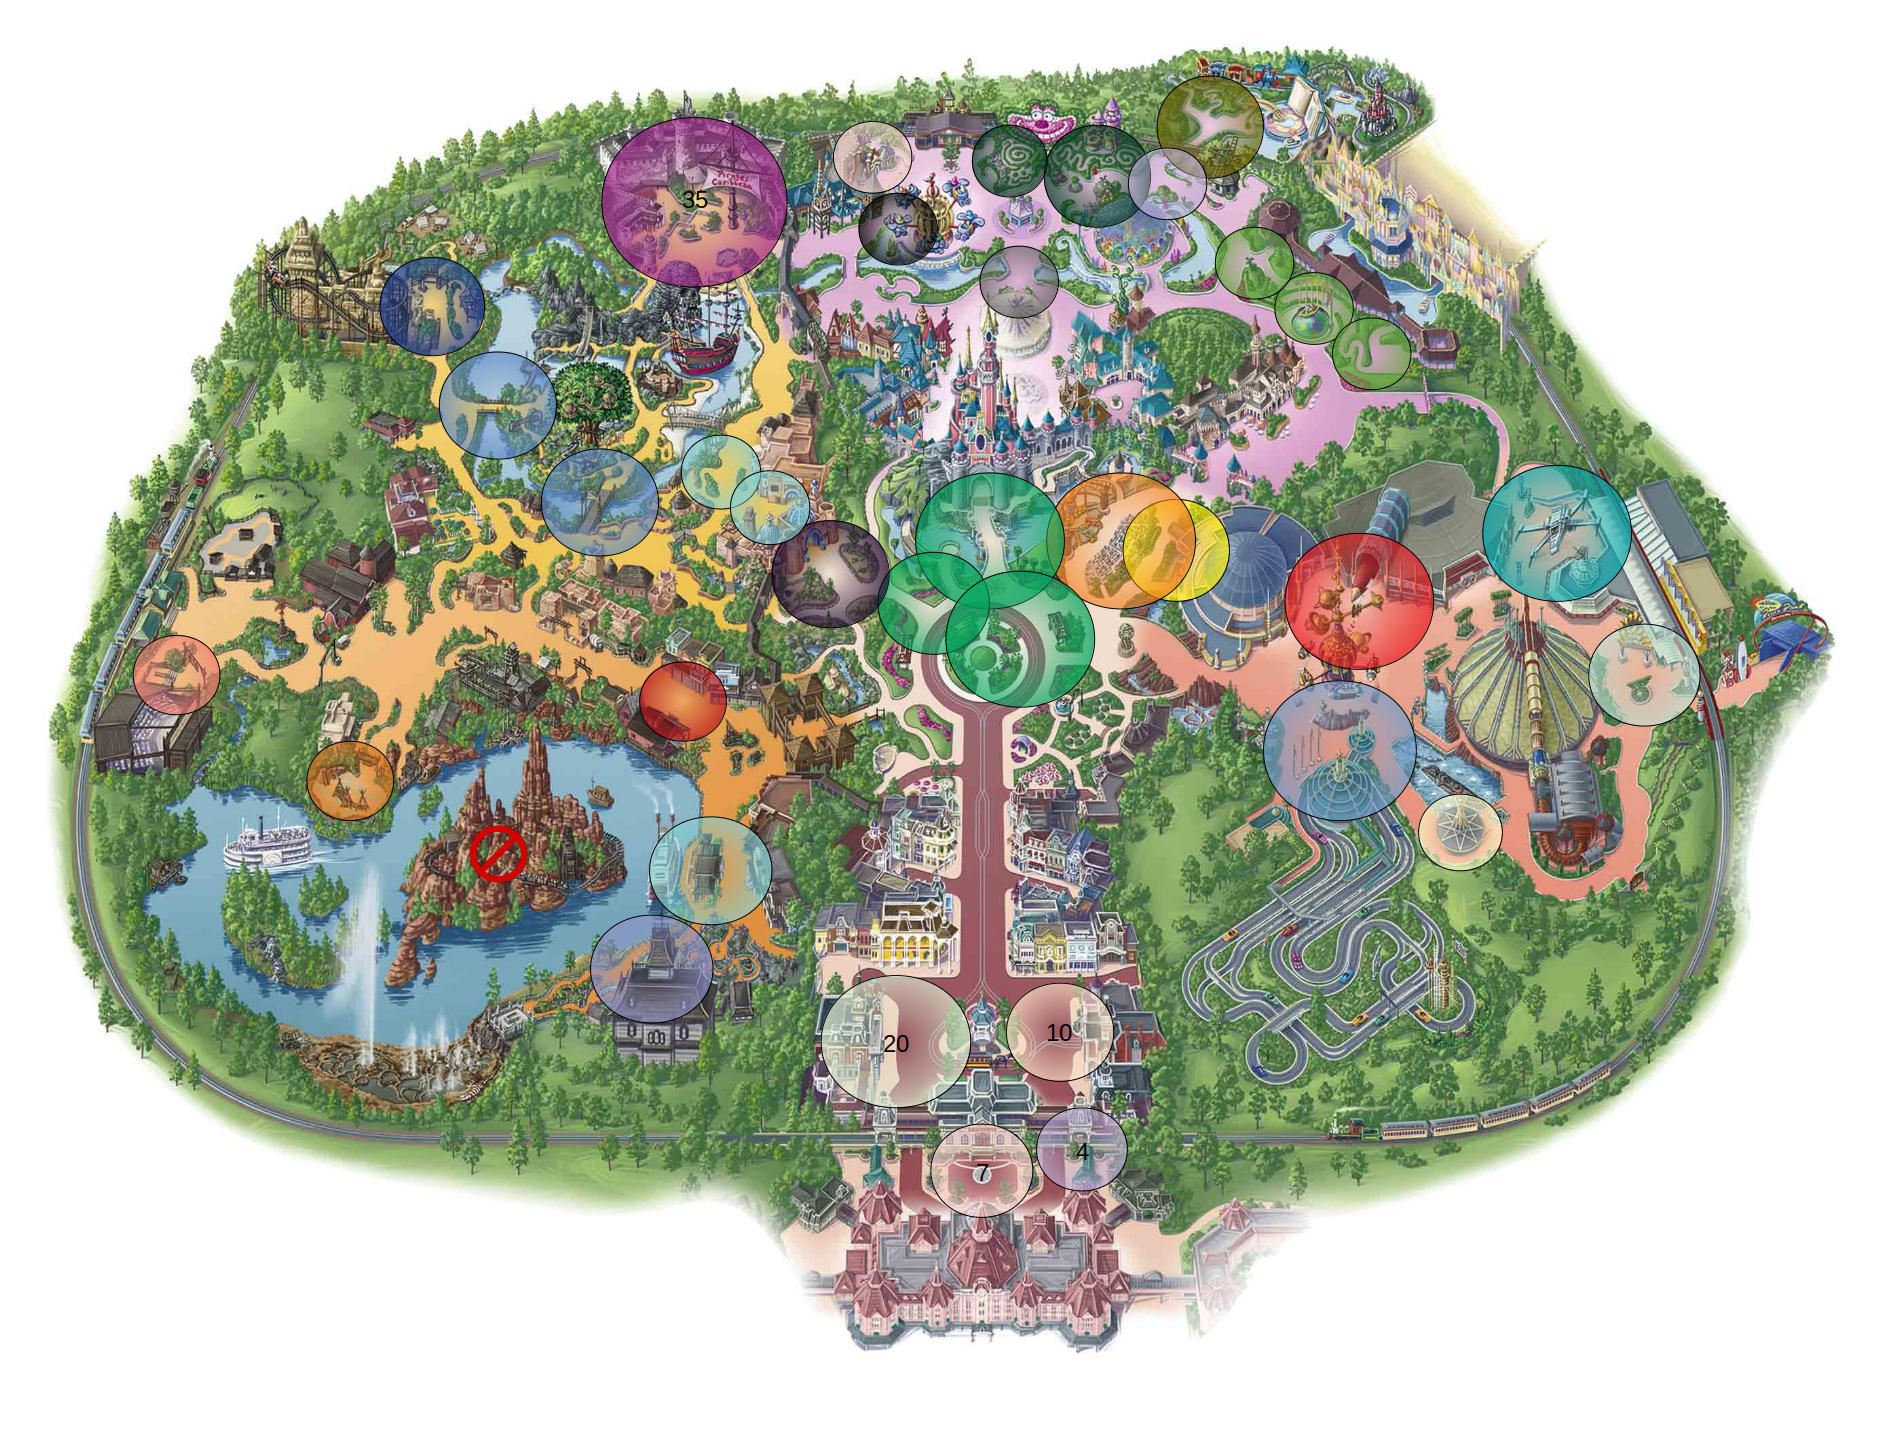
\includegraphics[width=0.5\textwidth]{imatges/zones_candidates.png}\par\vspace{1cm}
	\caption{Mapa amb les zones candidates}.
	\label{fig:zones_candidates}
\end{figure}

\subsection{Ubicar els restaurants}

Una vegada definida les zones candidates, realitzem totes les possibles combinacions dels restaurants en les zones candidates i calculem el benefici de cada restaurant donada la zona. 

Una vegada generada totes les combinacions, ens quederem amb el benefici més gran i ja sabem les ubicacions de tots els restaurants.

Podem visualitzar un exemple d'una solució a la figura \ref{fig:mapa_restaurants}.

\begin{figure}[h]
	\centering
	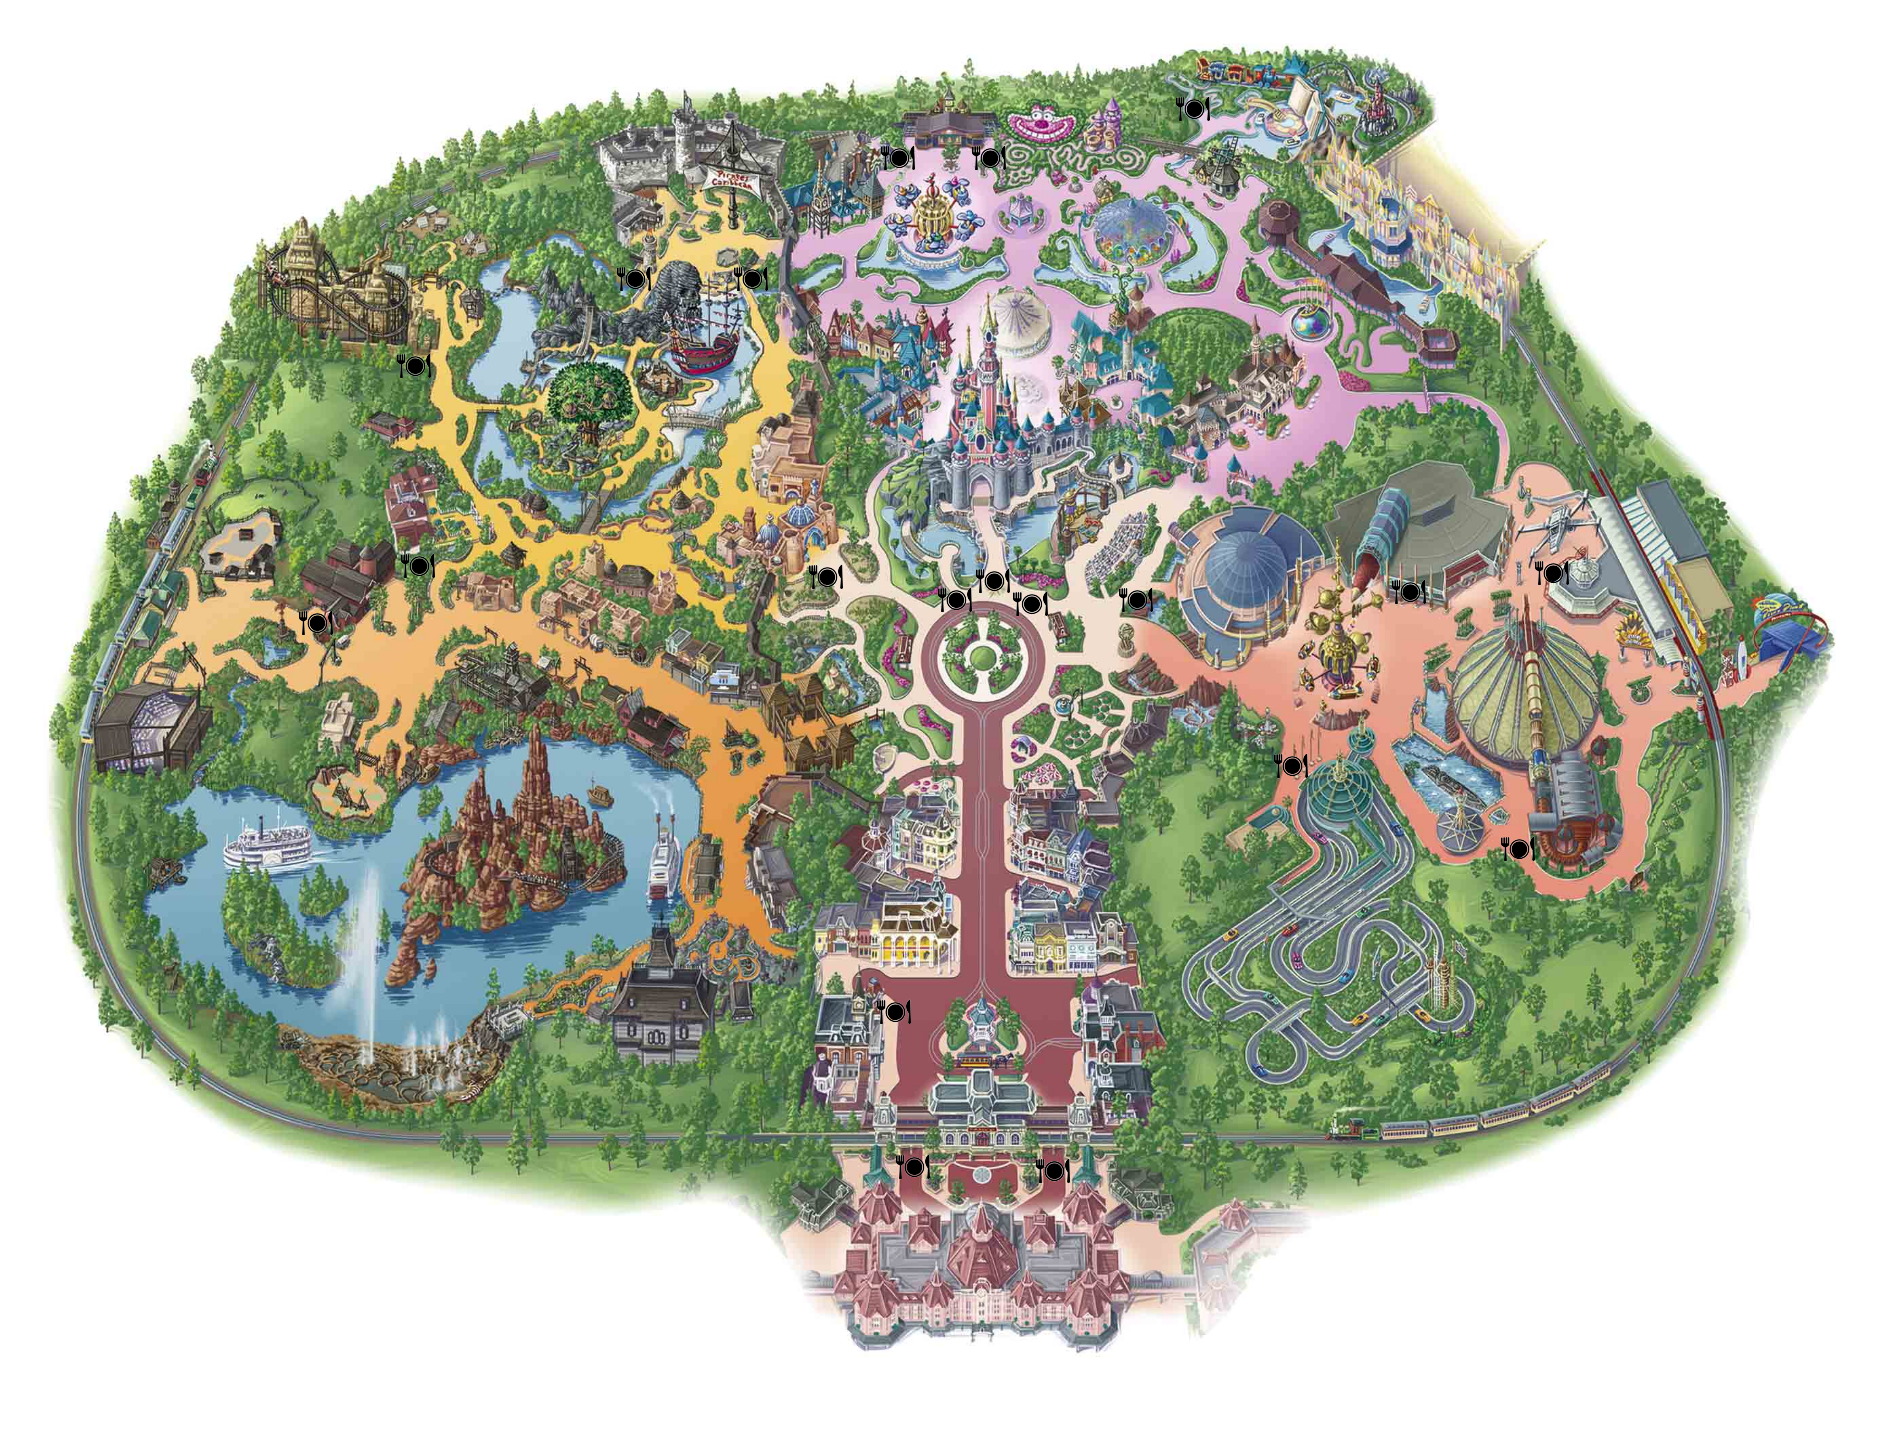
\includegraphics[width=0.5\textwidth]{imatges/mapa_restaurants.png}\par\vspace{1cm}
	\caption{Mapa d'atraccions amb les ubicacions dels restaurants}.
	\label{fig:mapa_restaurants}
\end{figure}


\section{Pre-processament de dades}
%Bla bla bla
Pel caràcter del problema i per evitar errors, realitzarem un preprocessament amb els punts recollits, de tal manera que, només considerarem els punts que:
\begin{itemize}
	\item S’han recollit dins d’un conjunt de franges horàries que considerarem de interés pels visitants alhora de buscar un restaurant per anar a menjar. 
	Així doncs, el llistat de franges horàries per les dades a considerar és:
	\begin{itemize}
		\item Esmorzar: 9h-10h
		\item Dinar: 12h-14h
		\item Berenar: 17h-18h
		\item Sopar: 20h-22h
	\end{itemize}

	\item No s’hagin recollit a les zones on es troben obstacles. 
	Considerem obstacles a les atraccions, boscos, llacs….
\end{itemize}


%\subsection{Algoritme}

\clearpage
\section{Articles}

%\clearpage
%\section{Treball futur}

%\clearpage
%\section{Conclusions}

\clearpage
\section{Bibliografia}
\clearpage
\end{document}
